\begin{section}{SC}{cosmological radiative transfer for Adaptive Mesh
    Refinement\\ simulations}
  \begin{minipage}[l]{\textwidth}

    {\small We present a new three-dimensional radiative transfer (RT) code,
      RADAMESH, based on a ray-tracing, photon-conserving and adaptive (in space
      and time) scheme. RADAMESH uses a novel Monte Carlo approach to sample the
      radiation field within the computational domain on a "cell-by-cell" basis.
      Thanks to this algorithm, the computational efforts are now focused where
      actually needed, i.e. within the Ionization-fronts (I-fronts). This
      results in an increased accuracy level and, at the same time, a huge gain
      in computational speed with respect to a "classical" Monte Carlo RT,
      especially when combined with an Adaptive Mesh Refinement (AMR) scheme.
      Among several new features, RADAMESH is able to adaptively refine the
      computational mesh in correspondence of the I-fronts, allowing to fully
      resolve them within large, cosmological boxes. We follow the propagation
      of ionizing radiation from an arbitrary number of sources and from the
      recombination radiation produced by H and He. The chemical state of six
      species (HI, HII, HeI, HeII, HeIII, e) and gas temperatures are computed
      with a time-dependent, non-equilibrium chemistry solver. We present
      several validating tests of the code, including the standard tests from
      the RT Code Comparison Project and a new set of tests aimed at
      substantiating the new characteristics of RADAMESH. Using our AMR scheme,
      we show that properly resolving the I-front of a bright quasar during
      Reionization produces a large increase of the predicted gas temperature
      within the whole HII region. Also, we discuss how H and He recombination
      radiation is able to substantially change the ionization state of both
      species (for the classical Stroemgren sphere test) with respect to the
      widely used "on-the-spot" approximation.}
  \end{minipage}

  \vspace{0.5cm}

  \begin{minipage}{\linewidth}
    \begin{center}
      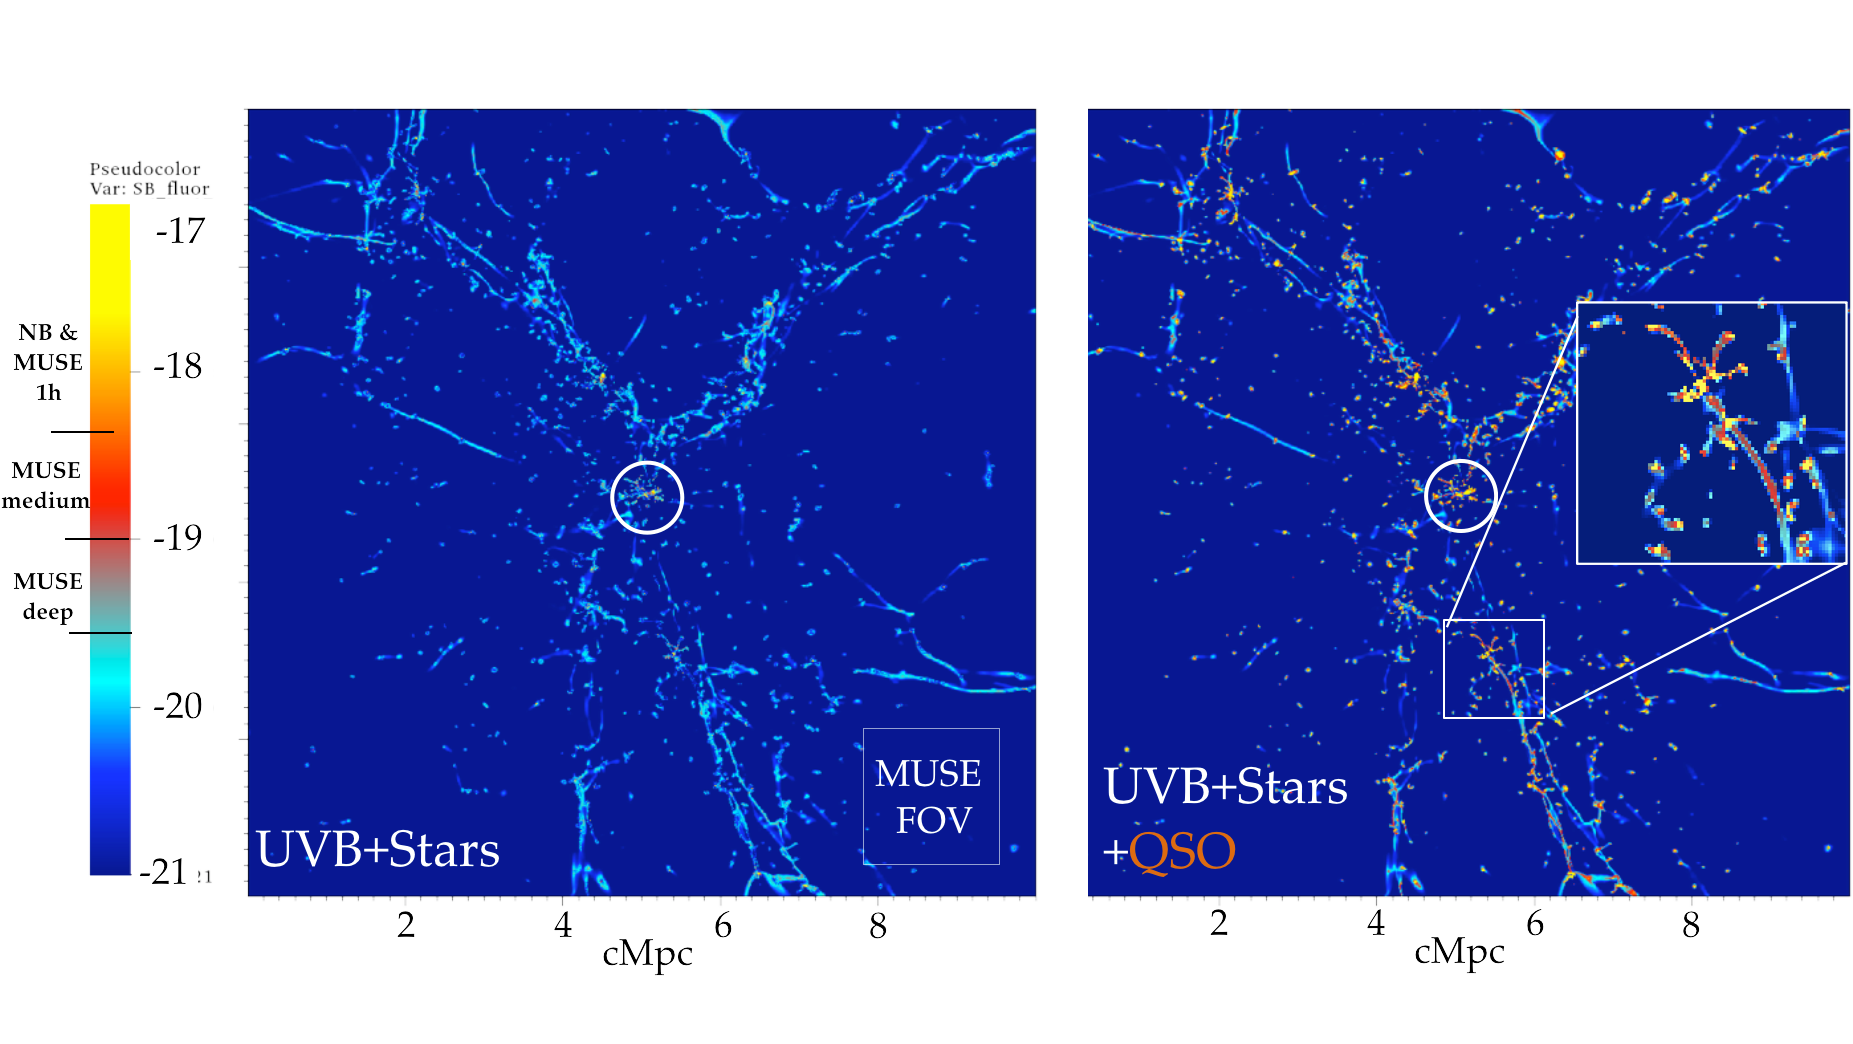
\includegraphics[height=15cm]{SC/Radamesh.png}
    \end{center}
  \end{minipage}

  \vspace{0.5cm}

  {\footnotesize \textit{[Cantalupo, S \& Porciani, C 2011, 2011MNRAS.411.1678C]}}
\end{section}